\chapter{Analyse van het probleem}
\label{Analyse_van_het_probleem}
%%%%%%%%%%%%%%%%%%%%%%%%%%%%%%%%%%%%%%%%%%%%%%%%%%%%%%%%%%%%%%%%%%%%%%%%

\begin{center}
    \begin{minipage}{0.5\textwidth}
        \begin{small}
            Waar de noodzaak van dit project word blootgelegd, door het probleem te analyseren.
        \end{small} 
    \end{minipage}
    \vspace{0.5cm}
\end{center}

Om door middel van de CCS standaard te kunnen DC snelladen is een communicatie
koppeling nodig tussen de \ac{ev} en de \ac{evse}. Deze koppeling is nodig om
onder anderen de gewenste laadstroom door te geven aan de \ac{evse}. De CCS
standaard gebruikt een powerlijn communicatie protocol waarvoor een \ac{modem}
nodig is. Ook moet er zowel in de \ac{ev} als in de \ac{evse} door een state
machine worden gelopen. En in geval van noot moet de lader gecontroleerd, of
ongecontroleerd kunnen woorden losgekoppeld van de \ac{evse}. Dit staat
allemaal beschreven in ISO 15118 waar CCS op gebaseer is \cite{15118}.

%%%%%%%%%%%%%%%%%%%%%%%%%%%%%%%%%%%%%%%%%%%%%%%%%%%%%%%%%%%%%%%%%%%%%%%%
\section{Wat is CCS DC snel laaden?}
%%%%%%%%%%%%%%%%%%%%%%%%%%%%%%%%%%%%%%%%%%%%%%%%%%%%%%%%%%%%%%%%%%%%%%%%

Als een accupakket met CCS DC word geladen, dan worden de polen van het
accupakket direct aangesloten op de \ac{evse}. Er moeten wel enkelen stappen
worden doorlopen voordat dit contact kan worden gemaakt. Zo moet communicatie
tussen de \ac{ecu} in de \ac{ev} en de \ac{evse} worden bewerkstelligd, waarmee
de \ac{ecu} de gewenste spanning van de \ac{evse} kan vragen. Na een aantal
checks kunnen de CCS contactoren (zie figuur \ref{fig:CCS_HV_diagram}) dicht
worden gedaan. Als de CCS contactoren dicht zijn, kan de \ac{ecu} stroom gaan
vragen van de \ac{evse}. Dan moet de \ac{ecu} de stroom gaan variëren
afhankelijk van de \ac{soc}, de temperatuur en de \ac{soh} van het accupakket.

\begin{figure}[h]
    \centering
    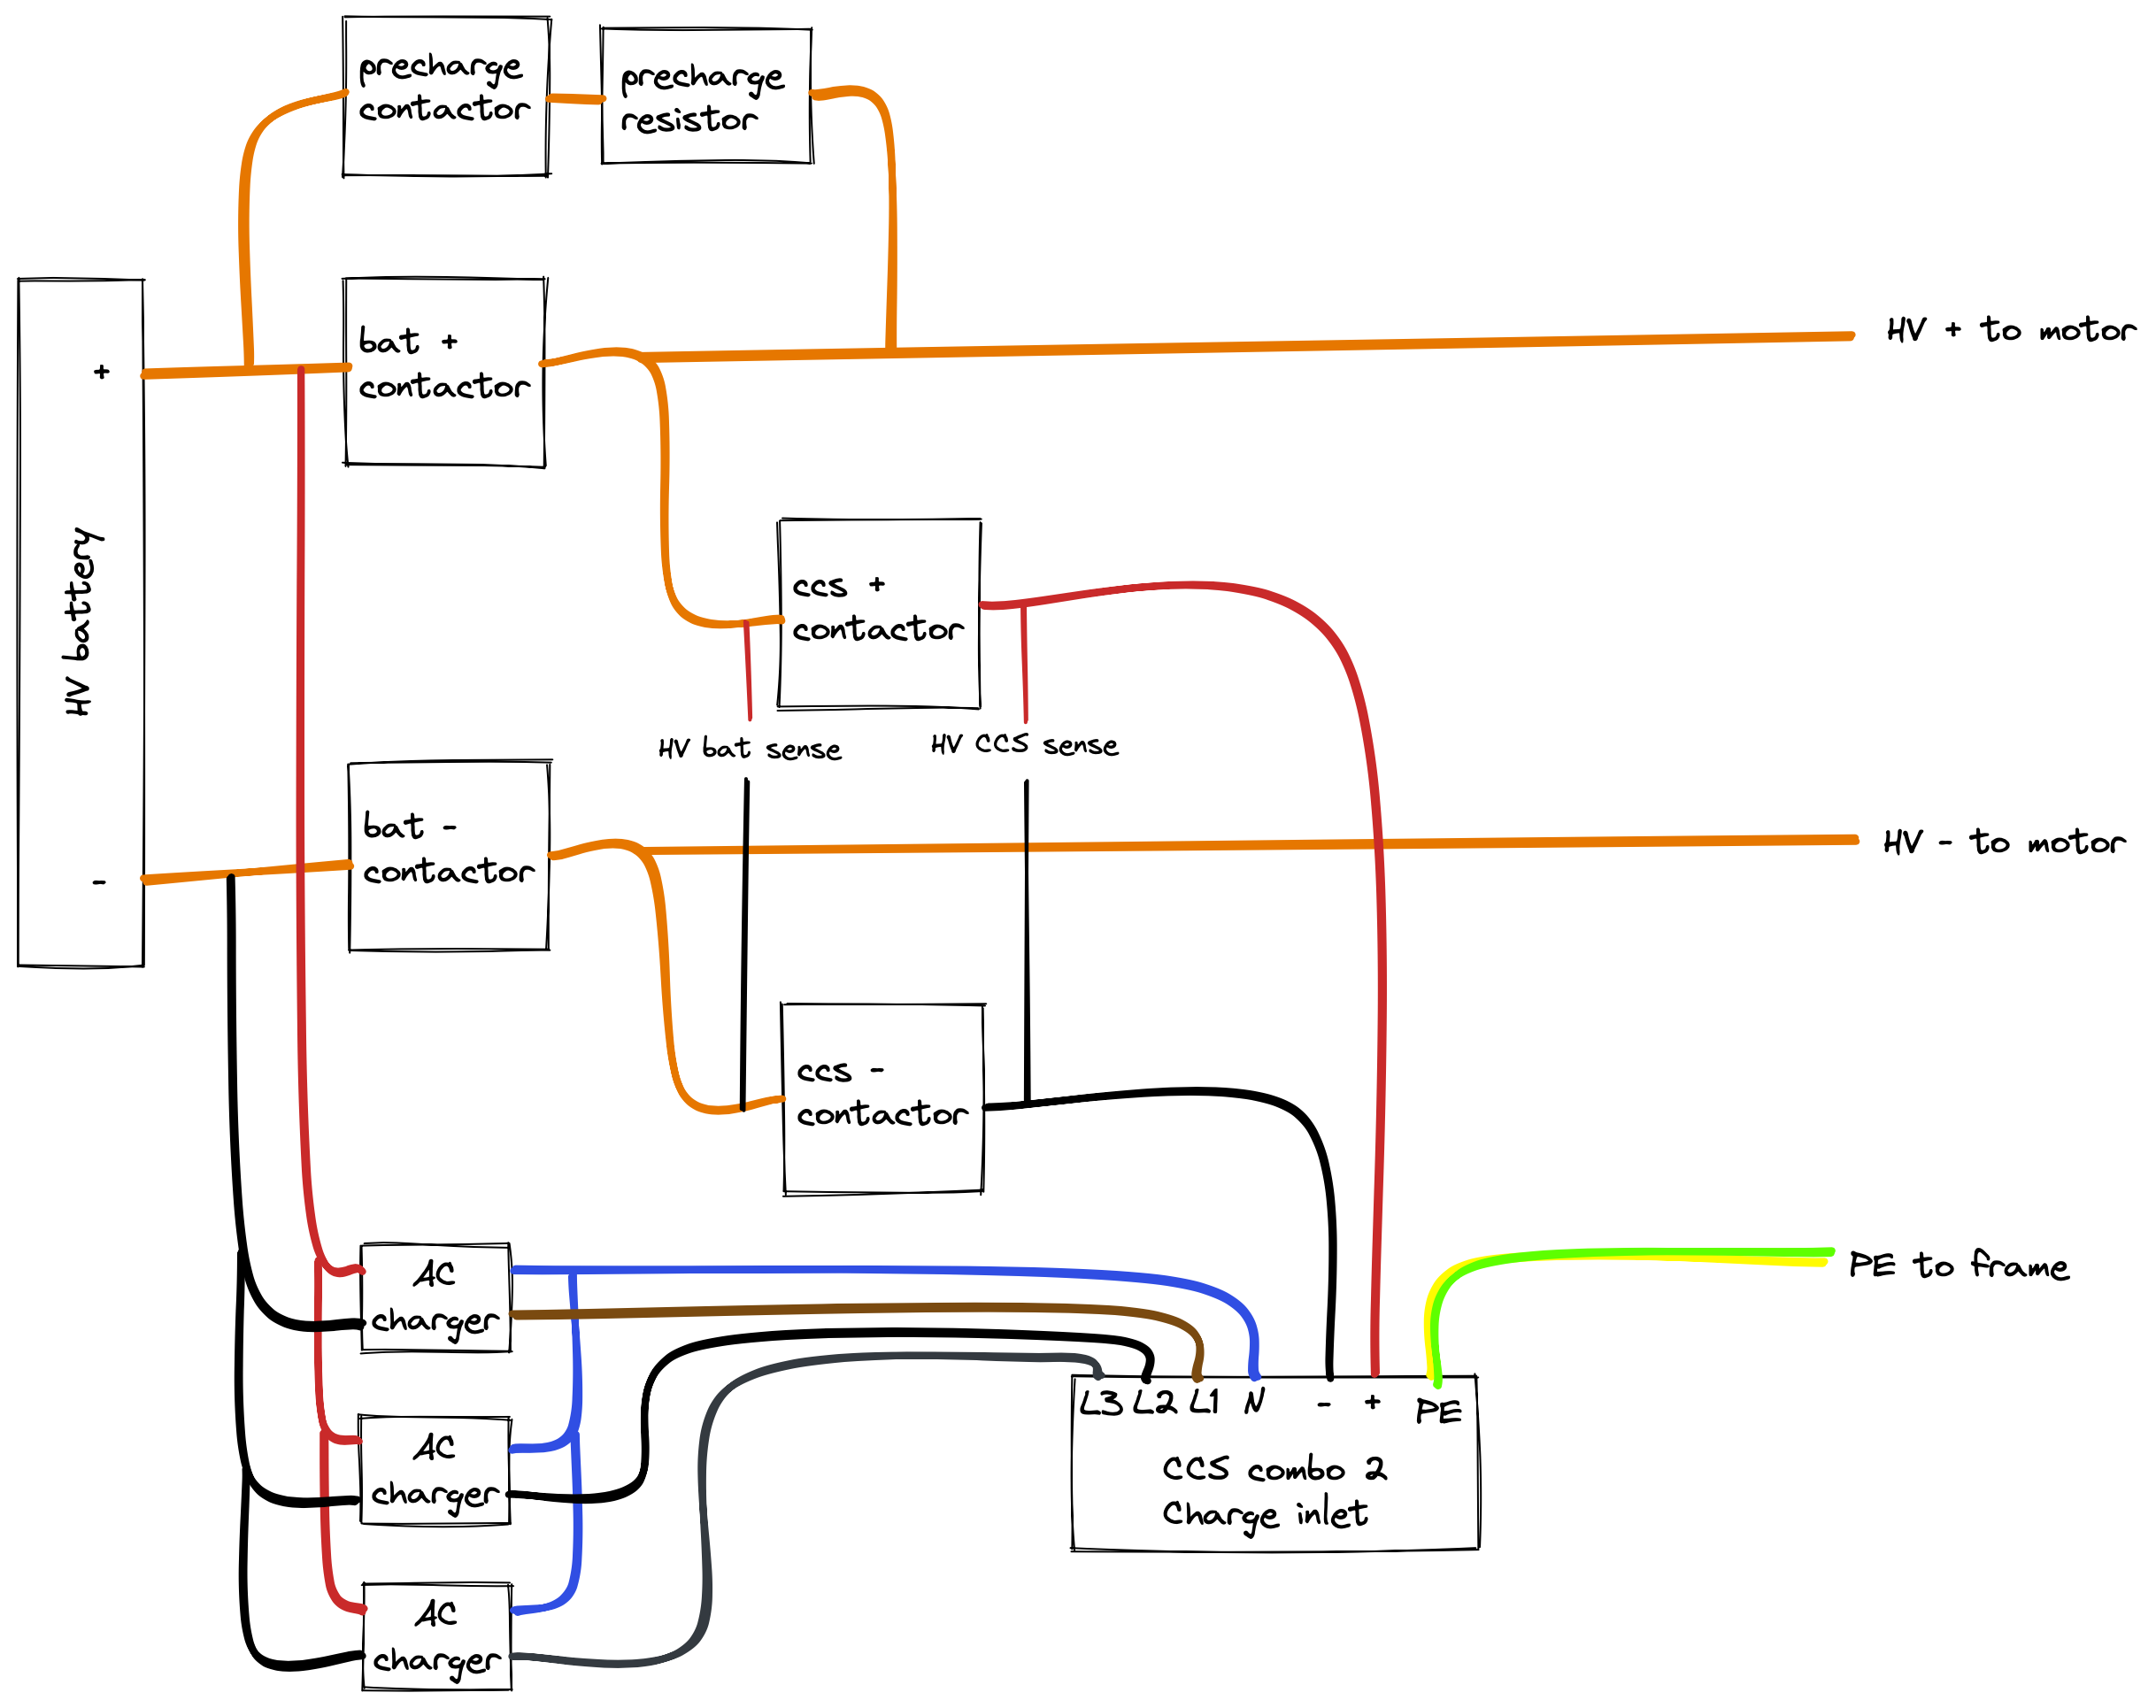
\includegraphics[width=0.85\textwidth]{CCS_HV_diagram}
    \caption{CCS DC snel laaden \ac{hv} diagram}
    \label{fig:CCS_HV_diagram}
\end{figure}

%%%%%%%%%%%%%%%%%%%%%%%%%%%%%%%%%%%%%%%%%%%%%%%%%%%%%%%%%%%%%%%%%%%%%%%%
\subsection{Voordelen van CCS DC snel laaden}
%%%%%%%%%%%%%%%%%%%%%%%%%%%%%%%%%%%%%%%%%%%%%%%%%%%%%%%%%%%%%%%%%%%%%%%%

Het voornaamste voordeel van \ac{dc} laden is dat je veel sneller kan laden dan
op \ac{ac}. Dat komt doordat bij \ac{ac} laden de limiterende factoren de
capaciteit van de aan board ladders zijn, of de maximaale stroom die de
\ac{evse} of de infrastructuur  kan leveren. Met \ac{ac} laden wordt er
namelijk gebruikgemaakt van een lader die in de \ac{ev} zelf zit. En omdat daar
een aantal beperkingen aan zitten (gewicht, grote en temperatuur), kan die
lader niet zo snel laden als een lader (\ac{evse}) die "op het land" staat,
omdat hij die beperking niet heeft. 

%%%%%%%%%%%%%%%%%%%%%%%%%%%%%%%%%%%%%%%%%%%%%%%%%%%%%%%%%%%%%%%%%%%%%%%%
\subsection{Beperkingen van CCS DC snel laaden}
%%%%%%%%%%%%%%%%%%%%%%%%%%%%%%%%%%%%%%%%%%%%%%%%%%%%%%%%%%%%%%%%%%%%%%%%

CCS laden vereist extra elektronica in de \ac{ev} en een combo 2 inlet. Ook is
een minimale accu spanning van \si{200\volt} nominaal nodig. Daarom kan niet elke auto
gebruikmaken van CCS.

%%%%%%%%%%%%%%%%%%%%%%%%%%%%%%%%%%%%%%%%%%%%%%%%%%%%%%%%%%%%%%%%%%%%%%%%
\section{Wat moet er ontwikkeld worden}
%%%%%%%%%%%%%%%%%%%%%%%%%%%%%%%%%%%%%%%%%%%%%%%%%%%%%%%%%%%%%%%%%%%%%%%%

Voor CCS DC snel laaden moet er een modum worden ontwikkeld. En een CCS
controller dat moet comunniceren met de \ac{evse} en het \ac{bms} van de
\ac{ev}. Dit moet ook een state machine zijn die de \ac{evse} kan aanroepen en
de laadstroom terug comunnceert met de \ac{evse} afhankelijk van de \ac{soc},
de temperatuur en de \ac{soh} van het accupakket. Ook met er electronica koomen
die de CCS contactoren aanstuurt en de batterij en CCS spanning meet.
